\documentclass[../AbiMappe_Mathe.tex]{subfiles}

\begin{document}

\theoremstyle{nonumberplain}

\newframedtheorem{fmytheo2}{}

%qlmanage -t -s 1000 -o . picture.svg 

\section{Naive Mengenlehre}
Eine Menge ist eine Zusammenfassung von wohlbestimmten Objekten zu einem Ganzen.
Diese Objekte heissen Elemente.\\\\
\textbf{Elementbeziehung}\\
Sei $M$ eine beliebiege nichtleere Menge dann bedeutet, $x \in M$, das wir ein beliebiges $x$ der Menge $M$ auswaehlen.

\subsection{Angabe von Mengen}
\textbf{Aufzaehlung:}\\
Eine endliche Menge kann durch aufzaehlung all ihrer Elemente angegeben werde z.B. stellt\\ $M=\{1,2,3,4,5\}$, die Menge aller natuerliche Zahlen $<6$ dar.\\\\
\textbf{Bildungsgesetz:}\\
Eine unedliche Menge kann mit Hilfe eines Bildungsgesetzes angegeben werden z.B. \\$M=\{1,2,3,\dots\}=\mathbb{N}$\\\\
\textbf{Eigenschaft:}\\
Eine Teilmenge $M$ einer Menger $N$ kann mit Hilfe einer Eingenschaft $E$ die alle Elemente der Menge entweder besitzen oder nicht angegeben werden $M=\{x \in N|E(x)\}$

\subsection{Mengenbeziehungen}

\subsubsection{Teilmenge:}
\textbf{Definition:} Sei M eine Menge. Dann heisst eine weitere Menge N Teilmenge von M wenn gilt:
\begin{align*}
x \in N \Rightarrow x \in M
\end{align*}
\textbf{Notation:} 
\begin{align*}
N \subseteq M
\end{align*}


\subsubsection{Potenzmenge}
\textbf{Defintion:} Sei $M$ eine Menge, dann nennt die Menge all ihrer Teilmengen $U$ Potenzmenge der Menge $M$.
\begin{align*}
\mathcal{P}(M) := \{U|U \subseteq M  \}
\end{align*}
\\\textbf{Beispiel:} 
\begin{align*}
\mathcal P&(\emptyset) = \{ \emptyset \}\\
\mathcal P&(\{ a \}) = \bigl\{ \emptyset, \{ a \} \bigr\}\\
\mathcal P&(\{ a, b \}) = \bigl\{ \emptyset, \{ a \}, \{ b \}, \{ a, b \} \bigr\}\\
\end{align*}

\subsubsection{Leere Menge}
\textbf{Definition:} Eine Menge $M$ die keine Elemente enhaelt nennt man leere Menge
\begin{align*}
M = \{\forall x:x\notin M\}  \Leftrightarrow: \emptyset
\end{align*}
\\
\textbf{Notation:}
\begin{align*}
\emptyset
\end{align*}

\subsubsection{Disjunktion(Vereinigung)}
\textbf{Definition:} Seien $N_1,N_2$ $\subseteq$ M, dann nennt man die Menge $X$ disjunktion(vereinigung) von $N_1$ und  $N_2$ wenn fuer alle $x \in X$ gilt, das $x \in N_1$ oder $x \in N_2$.
\begin{align*}
X=\{x \in M| x \in N_1 \lor x \in N_2 \}
\end{align*}
\\
\textbf{Notation:}
\begin{align*}
X=N_1 \cup N_2
\end{align*}
\\
\textbf{Venn-Diagramm}
\begin{figure}[H]
\centering
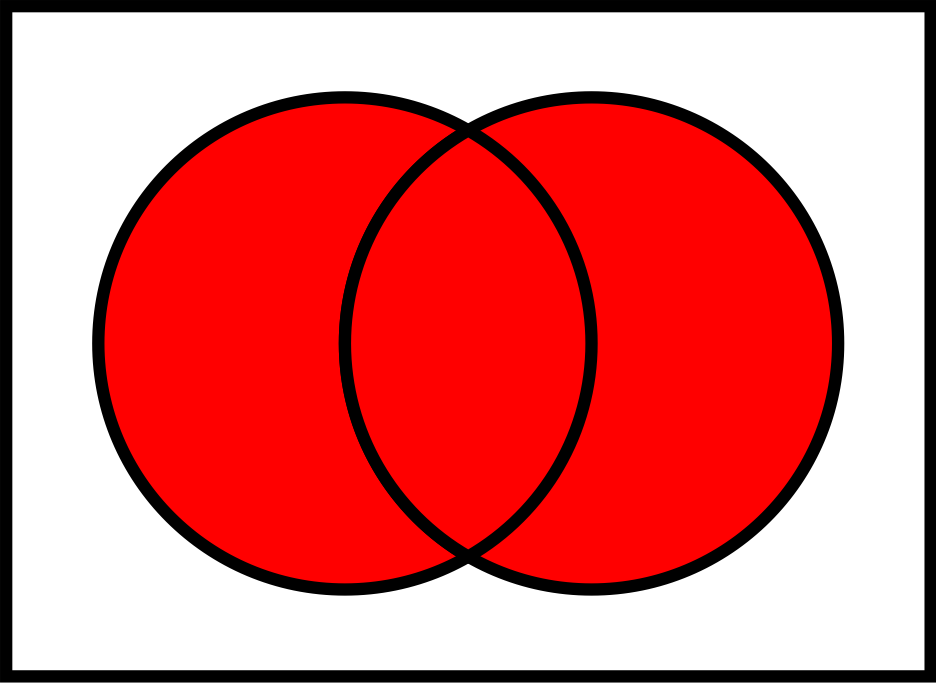
\includegraphics[width=117px, height=85.5px]{VennDis.png}
			% \captionsetup{labelformat=empty}
			% \caption{\label{fig:blue_rectangle} }
\end{figure}


\subsubsection{Konjunktion(Schnittmenge)}
\textbf{Definition:} Seien $N_1,N_2$ $\subseteq$ M, dann nennt man die Menge $X$ konjunktion(schnittmengen) von $N_1$ und  $N_2$ wenn fuer alle $x \in X$ gilt, das $x \in N_1$ und $x \in N_2$.
\begin{align*}
X=\{x \in M| x \in N_1 \land x \in N_2 \}
\end{align*}
\\
\textbf{Notation:}
\begin{align*}
X=N_1 \cap N_2
\end{align*}
\\
\textbf{Venn-Diagramm}
\begin{figure}[H]
\centering
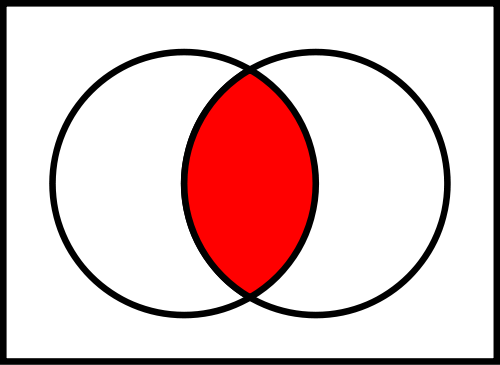
\includegraphics[width=117px, height=85.5px]{VennKon.png}
			% \captionsetup{labelformat=empty}
			% \caption{\label{fig:blue_rectangle} }
\end{figure}


\end{document}